\subsection{The trpzip2 $\beta$-peptide.}
\label{applications:hairpin}

\begin{figure*}[tb]
  \begin{center}
    \resizebox{\textwidth}{!}{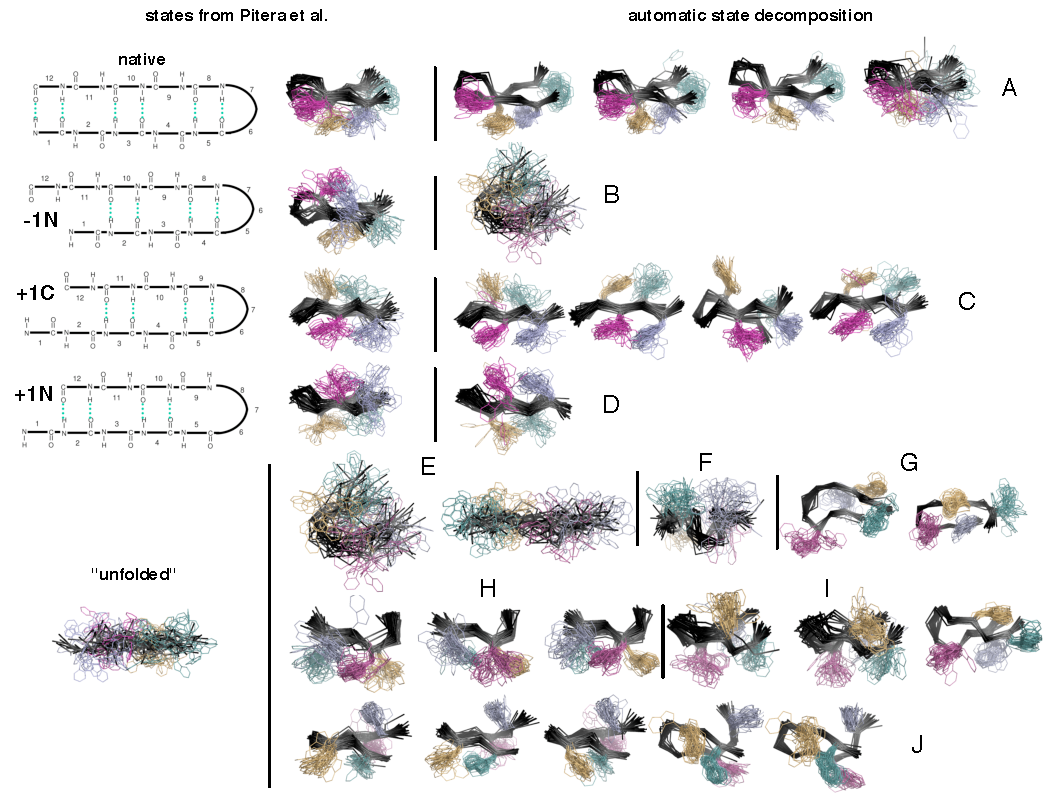
\includegraphics{chapters/automatic-state-decomposition/figures/trpzip2/comparison-with-reptated-states.pdf}}    
  \end{center}
  \caption{{\bf Comparison of some trpzip2 macrostates found by automatic state decomposition with misregistered hydrogen bonding states identified in a previous study.}  
  Left: The five hydrogen bonding patterns enumerated in Pitera \emph{et al.\ } \cite{pitera:2006a} that occurred in sufficient numbers in the subsampled trpzip2 dataset used here, with representative conformational ensembles.  
  Right: A selection of macrostates discovered by automatic state decomposition that the contain the largest numbers of hydrogen bonding pattern states.  
  The backbone is depicted in alpha carbon trace, and tryptophan sidechains are shown in light blue (Trp2), orange (Trp4), magenta (Trp9), and teal (Trp11).
  A complete set of macrostates obtained from the 40-state decomposition of the trpzip2 dataset is available as Supplementary Information.
  }
  \label{figure:trpzip2-states}
\end{figure*}

\begin{figure}[tbp]
  \begin{center}
    \resizebox{3.375in}{!}{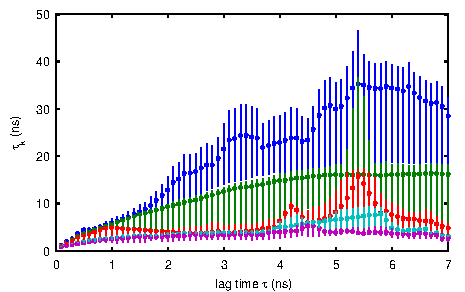
\includegraphics{chapters/automatic-state-decomposition/figures/trpzip2/trpzip2-timescales.pdf}}    
  \end{center}
  \caption{{\bf Implied timescales of trpzip2 as a function of lag time for 40-state automatic state decomposition.}  The five longest timescales are show.  Vertical bars depict 68\% confidence intervals.}
  \label{figure:trpzip2-timescales}
\end{figure}

As an illustration of the application of the state decomposition algorithm to a system with complex kinetics implying the existence of multiple metastable states \cite{yang:2004c}, we considered the engineered 12-residue $\beta$-peptide trpzip2 \cite{cochran:2001a}.
A set of 323 10 ns constant-energy, constant-volume simulations of the unblocked peptide\footnote{Note that the peptide studied experimentally in Refs. \cite{cochran:2001a} and \cite{yang:2004c} was synthesized with an amidated C-terminus, whereas the termini of the simulated peptide in the dataset considered here were left zwitterionic.} simulated using the AMBER parm96 forcefield \cite{AMBER-parm96} in TIP3P water \cite{jorgensen:1983a} was obtained from Pitera et al.\ \cite{pitera:2006a}; 
details of the simulation protocol are provided therein.
The trajectories were initiated from an equilibrium sampling of configurations at 425 K, a temperature high enough to observe repeated unfolding and refolding events at equilibrium.
Configurations were sampled every 10 ps, giving a total of 3.23 $\mu$s of data in 323 000 configurations.

The automatic state decomposition method was applied to obtain a set of 40 macrostates in 10 iterations of splitting and lumping.
In the first iteration, the conformations were split into 400 microstates, and in subsequent iterations, as described in Section \ref{section:methods:implementation}.

Figure \ref{figure:trpzip2-states} depicts some of the final set of 40 macrostates compared with a set of states produced by consideration of backbone hydrogen bonding patterns in a previous study by Pitera \emph{et al.} \cite{pitera:2006a}.
(The complete set of macrostates is shown in a figure included as Supplementary Information.)
As the trajectories considered here were resampled to 10 ps intervals (rather than 1 ps in Ref. \cite{pitera:2006a}) we found less than five examples of the +2 and -2 hydrogen bonding states identified in Ref. \cite{pitera:2006a}, and therefore do not include them in the comparison.
The automatic state decomposition method recovers states corresponding to the native, +1C, and +1N hydrogen bonding patterns, and often further separates conformations based on the packing of the tryptophan sidechains (Figure \ref{figure:trpzip2-states}, A, C, D).
However, the -1N hydrogen bonding pattern is not further resolved, and instead is grouped into a state of mostly disordered hairpins; further examination is necessary to determine whether the algorithm simply failed to resolve this state or if the state is simply not long-lived.
% JDC: Nina will check integrated correlation time of this state.
% NS: John, I *think* I know the correspondence between jed's state numbers and the hydrogen bonding pattern, but I enumerated it below just in case
% NS: Since some of the states were so small, they had zero count for their self-transition probability at some lag times.  This caused imaginary values when I took the log to estimate the exponential fit, so I didn't include them in the exponential fit, and used the fit in the correlation time calculation instead of the real value.  This did not change any of the helix correlation times since ever had zero counts.
% NS: state 1 (native) - tau = 1713.3 (in 10ps) = (17 ns?)
% NS: state 2 (unfolded) - tau = 1414.8 (in 10ps) = 14 ns
% NS: state 3 -- no examples
% NS: state 4 (-1N) - tau - 91.6 (in 10ps) = .9 ns 
% NS: state 5 (+1C) - tau - 235.8 = 2.4 ns
% NS: state 6 (+1N) - tau - 817.6 = 8.2 ns
% NS: state 7 (too unreliable)
% NS: state 8 (too unreliable)
In addition to recovering most of the manually identified misregistered states, the algorithm was also able to greatly resolve the state labeled as ``unfolded'' in Pitera \emph{et al.} (in that it did not conform to any of the enumerated hydrogen bonding patterns) into substates which exhibit considerable structure (E--J).
Some of these kinetically resolved states have distinct hydrogen bonding patterns, such as where both strands are rotated (H), causing the tryptophan sidechains to appear on the opposite face, or where the misregistration is greater than two residues (G, J). 
% JDC: Check that these letters are right?
% NS: I don't know if J has large misregistration, is it easy to calculate hydrogen bonding patterns for a few conformations, since I have a hard time telling by eye.
This demonstrates the utility of the method in identifying additional kinetically relevant states that were not initially part of the experimental hypothesis space.

Figure \ref{figure:trpzip2-timescales} depicts the implied timescales of the kinetic model as a function of lag time.
The longest timescale ranges between 25 and 35 ns and appears to stabilize over the range of lag times considered, though the uncertainty is quite large.
Eigenvector analysis (described in Sec. \ref{section:theory:markov-model-introduction}) shows that this timescale corresponds to transitions between the unfolded and disordered hairpin states (E) and the hairpin with both strands rotated (H).
% JDC: Double-check?
% NS: I think that is right
The states labeled H together totaled 935 conformations, but appeared in only 13 trajectories, with over 95\% of the conformations appearing in a single trajectory.
% JDC: Which states?
% NS: The "H" states
Correlation time analysis (Sec. \ref{applications:helix}) suggests there are less than 10 independent samples for each of the three states, so proper resolution of this timescale would require more data.
% JDC: Fill in number.
% NS: There were also problems with the exponential fit since some states went to 1 at long lag times, causing the corr time to go to infinity.  I eglected these tau's as well.
% NS: State 10126 - tau = 115.3 (in 10 ps) = 1.2 ns, g = 232, 216 members --> number of trajectories = 6  
% NS: State 10503 - tau = 312.4 (in 10 ps) = 3.1 ns, g = 626, 446 members --> number of trajectories = 9
% NS: State 10772 - tau = 273.0 (in 10 ps) = 2.7 ns, g = 547, 273 members --> number of trajectories = 4
The second longest timescale grows to about 15 ns and levels off by around 4 ns, and corresponds to transitions between the unfolded and disordered hairpin states (E) and the 
% NS changed
% four states corresponding to \emph{native} in Figure \ref{figure:trpzip2-states}.
native backbone states (A).
The states involved in this transition are much better characterized, with a total of over 25 000 conformations appearing in over half the trajectories.
The next three longest timescales were all between 3 and 4 ns and correspond to movement between the unfolded state (E) and various sets of misregistered states, namely
%row 3 of the unfolded state, row 4 of the unfolded state, and the +1C state.
% NS deleted:
% reptated states G and I, and the +1C state (state C).
the newly identified misregistered states I and J, and the +1C state (C).
% JDC: Double-check these!
Unfortunately, these timescales are on the order of the Markov time for the whole system, so it is difficult to characterize these transitions well.
% JDC: Elaborate!

%\begin{itemize}
%%  \item Timescales
%%  \begin{itemize}
%%    \item Timescales (except for slowest) level off around 3 ns, suggesting a Markov time (internal equilibration time) of 3 ns.
%%    \item Slowest timescale at this point is unfolding/misfolding of bent/inside-out/all trp on back face hairpin.  (Two such states: 10042 and 10351.)  Timescale might be as long as 40 ns, but very low population state, and very little confidence in estimated timescale.  Can make a statement like ``90\% of snapshots in the state came from one or two trajectories''.
%%    \item Next-slowest timescale is much more robust, levels off, more well-determined.  Mostly transitions between folded unfolded/extended/collapsed hairpin with the two folded/native states. 20 ns timescale.
%%    \item Should we look up loosely-packed to well-packed native hairpin transition? - occurs on 1-3 ns timescale at 5ns lagtime
%%    \item Big gap in timescales, next slowest timescales correspond to unfolded to misfolded/reptated transitions, with timescales around 5 ns.  Can identify what some of these are.  
%%    \item Next-slowest timescale has one reptation, but sidechains of different member states are in different rotameric states.
%%  \end{itemize}
%  \item Time-evolution of model?
%  \item Main messages.
%   \begin{itemize}
%    \item We can pick up same states as Jed found manually, but done automatically.
%    \item Folding mechanism is same as Jed/Imran found: no reptation, misfolded states must unfold.
%    \item Slowest timescale may be unfolding from trap, but not enough data to be sure.  Next-slowest is folding.  Gap in timescales before faster aggregate timescales.
%   \end{itemize}
%   \item Something about how resulting model has some timescales faster than lag time, and might need to lump these out?
%   \item Could we compare these states with states we get from K-means, which are not kinetically meaningful?
%\end{itemize}
